\begin{bibunit}
\thispagestyle{plain}

% Add missing command definitions from original paper
\newcommand \op[1] {\ensuremath{\operatorname{\mathbf{#1}}}}
\newcommand \com[1] {\ensuremath{\mathtt{#1}}}
\newcommand{\RNum}[1]{\uppercase\expandafter{\romannumeral #1\relax}}

\section*{Abstract}
	In this paper, we discuss how process mining techniques can be applied in industrial control systems for modeling, verification, and enhancement of the cyber-physical system based on recorded data logs. Process mining is used for extracting the process models in different notations from the recorded behavioral traces of the system. The output model of the system’s behavior is mainly derived using an open-source tool called ProM. The model can be used for such applications as anomaly detection, detection of cyber-attacks and alarm analysis in industrial control systems with the help of various control flow discovery algorithms. The extracted process model can be used to verify how the event log deviates from it by replaying the log on Petri net for conformance analysis.
	
	\section{Introduction}
 
	Process mining \cite{van2012process1}  extracts the behavior of the system by analyzing the events in order and it consists of process discovery, conformance checking and process enhancement. Process models derived from event logs can be classified in different ways like how formal the model is, how the model is constructed, etc., and popular process modelling paradigms are Transition systems, Petri nets, Workflow nets, Business Process Modelling Notations (BPMN), Causal nets (C-nets),  etc. Data mining and process mining have some differences even if they used to predict patterns from data logs. Data mining is used to discover or predict the patterns by analyzing the data sets but process mining combines data analysis with modelling for extracting deep insights about the processes from recorded event logs  \cite{van2016process}. While data mining ignores the processes, process mining is really interested in processes using the data.
	
	There are three components in process mining technique \cite{van2012process2} i.e., process discovery, conformance checking and enhancement. The process discovery generates a model from a recorded event log with the help of several control flow discovery algorithms. The generated model and other event logs from the same system can be compared to identify the deviations this is called conformance checking. The generated model can be updated by analysing a new set of event logs called enhancement.
   
   Many process scenarios can be constructed by simulating the Petri net \cite{petri1962} and this method is called 'Play Out'. Instead of simulating the Petri net, we can use the simulation model or digital twins or even real systems to create the event log and inferring the model from many scenarios or traces is called process discovery or 'Play In'. It is possible to identify the deviation of the model by replaying a scenario on a built model. These features in process mining are helpful to identify bottlenecks in process and where machines deviate from expected process \cite{aalst2011process}.
   
   
	
	Cyber-physical systems (CPS) \cite{lee2017introduction} is a popular designation for complex industrial automation systems with decentralized control logic distributed across many communicating devices, often embedded into various mechatronic components. The IEC 61499 architecture \cite{iec61499part12012} is considered as a suitable method for modelling cyber-physical automation systems. In the modern automation industry world, mixed structure of distributed controllers in different mechatronic components introduces the verification and validation challenges, so formal modelling of CPS is necessary for their formal verification. The latter helps making the system less prone to errors by checking their behaviour comprehensively on compliance with specifications expressed in such formal languages, as temporal logic, e.g., LTL or CTL \cite{yoong2015verification}. Closed-loop modelling is considered beneficial for the verification but it requires the model of the plant. The implementation of the plant model is complex and resource consuming, and it is normally done by manually. The process mining approach opens a wide range of opportunities for modelling industrial control systems. In this paper, we discuss how process mining can be effectively applied in the field of industrial automation systems and it also describes the implementation of process model from event log by process discovery algorithm. Then we demonstrate how to check if the new event log deviates from the expected behaviour.
   
   
   The paper is structured as follows: Section \ref{sec:processmininginindustrialcontrolsystem}  discusses the related work and process mining in industrial control systems. Section \ref{sec:processmodelextraction} explains the event log structure, process mining tools and its advantages, selection of process discovery algorithms and conformance checking of process model in detail.  Finally, Section \ref{sec:conclusion} concludes the paper and outlines future goals.
   
   
   \section{Process mining in industrial control systems : Overview}
   \label{sec:processmininginindustrialcontrolsystem}
   \subsection{Process mining in factory automation}
   Process mining in industrial control systems can be applied in various directions. Process mining techniques applied in factory automation are used for model enhancement and conformance checking \cite{paper1}. The industrial control systems are used to record the events and this trace of events is called event log. The  event log can be in various formats like CSV, XES, MXML etc. The control work-flow model is discovered from the event log with the help process mining algorithms. There are several types of control flow discovery algorithms, but we need to select one of them according to the event log and depending on the goal of the process model. The model built by the process discovery algorithms is evaluated with the help of basic performance analysis which considers fitness, precision, over-fitting, and simplicity parameters. These parameters can be measured by replaying event log on derived model.
   
   \subsection{Anomaly detection using log data}
   
   Anomaly detection using log data found to be another application using process mining technique. Paper \cite{paper2} introduces a method for identifying anomalous behaviour of the industrial control system using device logs with the help of process discovery and conformance checking. Process mining techniques are mainly used in business related areas to improve the process by analysing the event log, but it is possible to detect cyber-attacks and anomalous behaviour of the industrial control system by analysing the event log using conformance checking. In the paper \cite{paper2}, process discovery algorithm generates process models which are used for conformance checking. The latter is done with the help of a token game which compares the new event log with the generated model. Myers found in \cite{paper3} that models created with the help of inductive miners give good fit compared to other miners, especially in the field of industry control system.
   
   \subsection{ Alarm analysis from the event-log database of an industrial plant}
   
   In industries alarm analysis can be done with the help of process mining techniques.  Abonyi and Dorgo explain in \cite{paper4} how process mining techniques can be used effectively for the alarm analysis from the event-log database of an industrial plant. Here, the process model is derived from fuzzy miner instead of the alpha miner \cite{van2004workflow} because alpha miner does not consider number of times the traces are repeated in event log while the fuzzy miner keeps the highly important behaviour of the system.
   
   \subsection{online parameter estimation for CPPS with process mining}
   
   In the cyber physical production systems (CPPS), the need to adjust in production entails the need to change the automation software which requires a lot of manual engineering effort. In order to fix this, paper \cite{paper5} provides online parameter estimation for a CPPS  using process mining. Alpha algorithm is one of the popular process discovery algorithms which creates dependency graphs from event logs. The dependencies between each event are created according to its order of events in the event log. If any noises present in the system, then the alpha algorithm produces a high difference from the expected behaviour \cite{paper5}.
   
   \subsection{PLC programming logic modelling and other applications in ICS }
   
   The alarm analysis, parameter estimation and detection of cyber-attacks in cyber physical systems based on outlier analysis in event logs were major application of the process mining. However,  Theis at al in \cite{paper6} propose a method to model PLC programming logic by analysing event log with the help of process mining. The paper uses split miner as a process discovery algorithm and uses DREAM-NAP (decay replay mining - next activity prediction) for predicting next activities in the running process. In the modern industry world robots help in the manufacturing system to increase the overall productivity of the processes. The data captured from the robots can be used to create a general model of the manufacturing system to understand and extract hidden behaviour of the system. The generated model and other event logs from the same system can be compared to identify the deviations. In this case, the process discovery algorithm inductive miner is used because it gives a more generalized model compared to other control flow discovery algorithms. Another paper \cite{paper8} which collects data from the factory floor and converts it to event stream in order to generate a model for conformance checking. The conformance checking detects deviation from the manufacturing floor.
   
   \subsection{Plant model generation from event log}
   
   In recent years, cyber physical systems are used in almost all wireless communication areas. These systems produce several flaws due to its decentralized and heterogeneous structure. Formal verification of these systems become more relevant in order to verify and detect possible errors in the system. Modelling of the controller is straightforward because logic is already known but the construction of plant model is difficult. Previously, the researchers manually constructed the model of the plant and used it for verification. The paper \cite{etfapaper} describes how to construct plant models automatically from event logs for formal verification. Formal model of the plant in SMV format is developed and verification is done with the help of a symbolic model checker tool called NuSMV.
   
   
   \section{Process model extraction}
   \label{sec:processmodelextraction}
   \begin{figure}[!t]
	   \centering
	   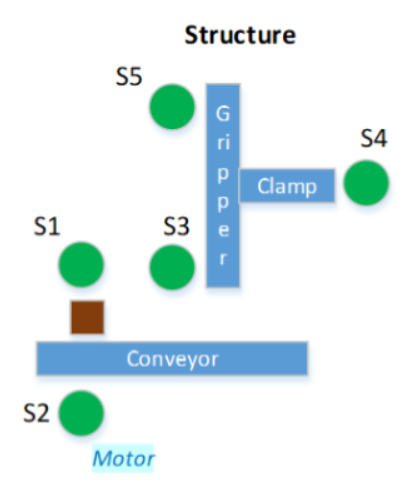
\includegraphics[width=0.3\textwidth]{MX_Papers/Paper5/images/structure.PNG}
	   \caption{Gripper and conveyor system structure}
	   \label{fig:structure}
   \end{figure}
   
   Consider a running example of  'Gripper and conveyor' system and see how the process flow of the system can be derived from the event log with the help of process discovery algorithms. The structure of the system is shown in the Figure \ref{fig:structure} consisting of a gripper and conveyor. Gripper can either move in 'upward' or 'downward' direction and the clamp attached to the gripper component can 'open' and 'close' to grab an object. The conveyor component moves in one direction when the actuator signal is triggered. There are five sensors and three actuators exists in the system and their description is given below:
   
   
   \subsubsection{Sensor signals} 
   \begin{itemize}
	 \item S1\_cup\_detected : Whenever a cup or an object appears in the sensor (S1) then its value will change to 'TRUE' otherwise its value remains the same as 'FALSE'. 
	 \item  S2\_conveyor\_running : If the conveyor is running then the sensor (S2) value becomes 'TRUE' otherwise 'FALSE'.
	 \item S3\_gripper\_at\_bottom : If the gripper's clamp reaches bottom position then the sensor (S3) value becomes 'TRUE' otherwise 'FALSE'.
	 \item S4\_gripper\_closed : Whenever clamp is closed then  sensor (S4) value will change to 'TRUE' otherwise its value remains same as 'FALSE'.
	 \item S5\_gripper\_at\_top : If the gripper's clamp reaches top position then the sensor (S5) value becomes 'TRUE' otherwise 'FALSE'.
   \end{itemize} 
   
   \subsubsection{Control signals}
   \begin{itemize}
	 \item C\_conveyor\_run : If the control signal becomes 'TRUE' then the conveyor starts running otherwise it stops.
	 \item  C\_gripper\_go\_down : If this signal becomes 'TRUE' then the gripper starts moving downwards otherwise it moves upward.
	 \item  C\_conveyor\_to\_close : If this signal becomes 'TRUE' then the clamp closes  otherwise it opens.
   \end{itemize}
   
   
   A simple process sequence is taken into account and it works cyclically for a particular period of time. Initially, the conveyor is moving, the gripper rests at top position and the clamp is already at open condition. Whenever 'CUP' (workpiece) is detected by sensor s1 then the conveyor stops running. Gripper comes down and grabs the 'CUP' with the help of its clamp. After that the gripper returns the 'CUP' on the conveyor and the conveyor moves again. This process runs cyclically and if there is no object then the conveyor keeps on running and the gripper does not do anything.
   
   \subsection{Event log structure, attribute selection and pre-processing}
   
   \begin{figure}[!t]
	   \centering
	   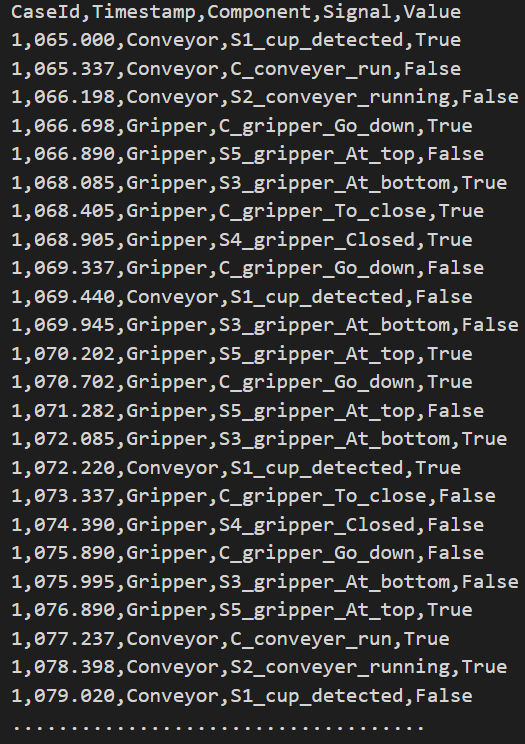
\includegraphics[width=0.3\textwidth]{MX_Papers/Paper5/images/EL.PNG}
	   \caption{Event log}
	   \label{fig:EL}
   \end{figure}
   
	An event description in the log consists of the following fields \cite{paper2}: case identifier, event id/name and attributes. The case identifier is a unique id for each execution of processes, Normally, industrial control system processes are cyclic so each cycle can be considered as a different process instance. The event name refers to the triggered activities that occur while running the system. The attributes’ part consist of resource, timestamp, etc. These attributes give additional information, i.e., ordering information, which component produced the event, etc. The attributes are not mandatory fields but if we get more information, then that would be useful to extract hidden features about the system.
   
	An event log of the 'Gripper Conveyor' system is shown in the Figure \ref{fig:EL} and it consists of five columns: CaseId, Timestamp, Components, Signal, Value. The case identifier in this log is denoted as 'caseId' which is a unique id for each process execution and here the event is composed of three columns: component, signal, and value. Timestamp represents the time at which the event occurred and it is considered as an attribute. This event log is taken as the input for further processing so it's necessary to record the correct information. The event log is sorted using 'Time Stamp' because the order of occurrence of events is a key factor and process discovery algorithms work mainly with the relation of these events.
	
	Event log should be cleaned to get a good quality event log. In many situations event log quality should not be compromised,  in order to produce an accurate model of the system. For anomaly detection, the log pre-processing step is ignored because these outliers or irrelevant events help to detect the cyber-attack while modelling the system with the help of process mining technique \cite{paper2}.
	
   
	\subsection{Process mining tools and its advantages}
   
   Process mining consists of process discovery algorithms and conformance checking can be done via programs, but process mining tools give wider option to use these all algorithms and it provides the result in different notation to give better visualization. ProM \cite{ProM} \cite{van2005prom} and Disco \cite{Disco} \cite{gunther2012disco} are the most popular tools used for process mining. ProM is an open-source tool which is is widely used because of the following features.
   
   
   ProM version 6 consists of 250+ plugins which are used for event log pre-processing, process discovery and visualizations. The representation of the process model can be expressed in different notations but most commonly represented as Petri nets. There are many process discovery algorithms \cite{van2009process} like Alpha, Alpha +, PL based, T alpha, Petrify miner, etc. to produce output models as Petri net and ProM tool which supports almost all of them. ProM also supports plugins for conformance checking, and LTL specification checking. The fitness of the model derived from event log can be analysed using conformance checking. The ProM framework has different plugins for basic performance analysis and these plugins help to identify how much the generated model deviated from event log. The event log analysis, log pre-processing, and conversion from one event log format to another like CSV to eXtensible Event Stream (XES) can be done easily with this tool. On the other hand, Disco, developed by Gunther in 2007, is based on the fuzzy miner algorithm.  The fuzzy miner gives a better interactive representation to understand the system behaviour of complex logs and it also works in the ProM tool.
   
   Most of the process discovery algorithms take input in XES format and produce process models. In order to convert the event log from CSV to XES format, the Standard XES attributes need to be mapped by selecting the ’Case’ columns, ’Event’ columns, ’Start Time’ column and ’Completion Time’ column from the CSV data log. In the ’Gripper Conveyor’ system the event log in CSV is converted by mapping the standard XES attributes as follows:
   
   
   \begin{itemize}
	 \item Selected Case Columns : CaseId
	 \item Selected Event Columns : Component, Signal and Value
	 \item Start Time \& Completion Time is not selected because timing information is not considered for this experiment.
   \end{itemize}
   
   \subsection{Selection of Process discovery algorithms }
   
   \begin{figure}[!t]
	   \centering
	   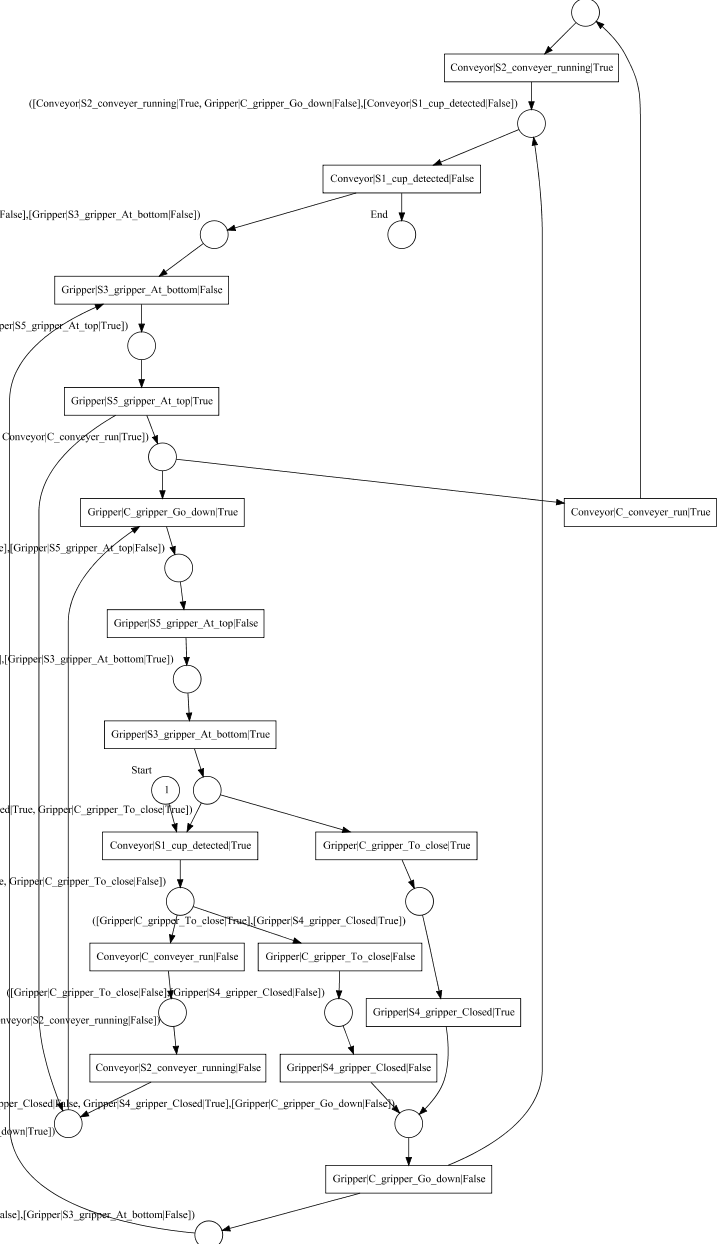
\includegraphics[width=0.5\textwidth]{MX_Papers/Paper5/images/PN.PNG}
	   \caption{Process model extracted using alpha algorithm in ProM}
	   \label{fig:PN}
   \end{figure}
   
   \begin{figure}[!t]
	   \centering
	   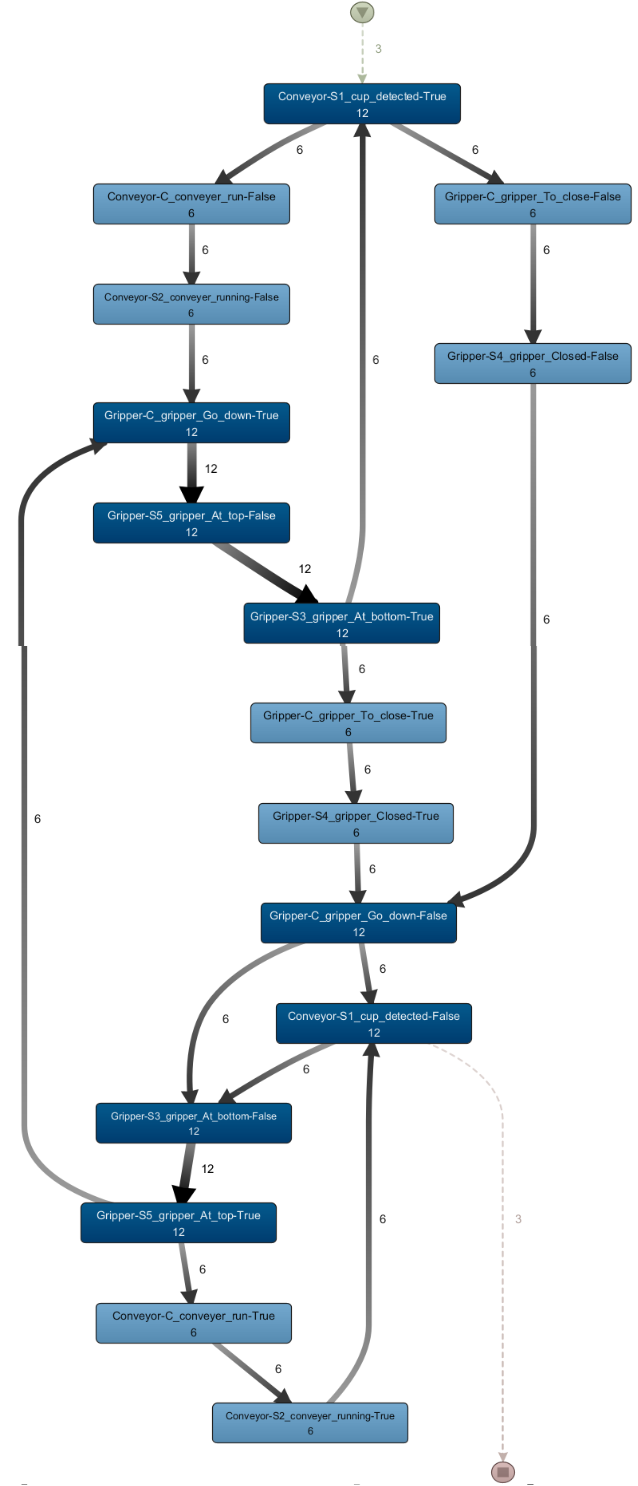
\includegraphics[width=0.37\textwidth]{MX_Papers/Paper5/images/disco.png}
	   \caption{Process model extracted using fuzzy miner in Disco}
	   \label{fig:fm}
   \end{figure}
   
   
	There are several types of process discovery algorithms: Abstraction based, Heuristic based, Search based, Region-based algorithms etc and each algorithm is used to extract different process models using event log. Abstract -based algorithms generate models by ordering relations of events in an event log, and on the other hand heuristic miner generates models where events are ordered based on frequency of events. Events happening in fewer thresholds are ignored so heuristic miners perform better with event logs containing noisy data. Search based algorithms (Genetic algorithm Miner (GA)) which try to mimic the process of evolution. Process discovery technique key factors is the balance between fitness, precision, generalisation and simplicity \cite{buijs2012role}. While selecting the process discovery algorithm, one should consider the following questions: how fast analysis technique produce result, how much memory it is used, what is representation of process discovery algorithm and whether it solves the related problems.
	
   
   The most commonly used process discovery algorithm is the alpha algorithm, which is an abstraction-based algorithm. The process model extracted from the event log \ref{fig:EL} of ’Gripper- Conveyor System’ using the alpha algorithm is shown in the Figure \ref{fig:PN} and it explains the process flow in the Petri net notation. The Petri net consists of 16 transitions and each transition denotes the activity from the event log. The alpha algorithm creates a dependency graph based on the order of events in the event log. It does not consider the frequency of trace, so noises present in the log makes a high difference from expected behaviour. In order to avoid this, we can use fuzzy miner which is a heuristic approach and it generates a model according to the frequency of the traces. According to  \cite{paper4}, ”the algorithm calculates the importance of the activities and how closely the events follow each other”. The process model extracted from the same ’Gripper Conveyor’ system using fuzzy miner in Disco is shown in the Figure \ref{fig:fm}. It is exactly similar to the Petri net obtained from the alpha algorithm. The fuzzy model can be approximated by changing its ’Activity’ and ’Path’ detail from 0 to 100 percentage and the thickness of edges in the graph explains the number of times the particular event to another event is occurred. The fuzzy model is difficult to convert to other process modelling languages but its representation is easy to understand system behavior.
   
   \subsection{Conformance checking}
   
   \begin{figure}[!t]
	   \centering
	   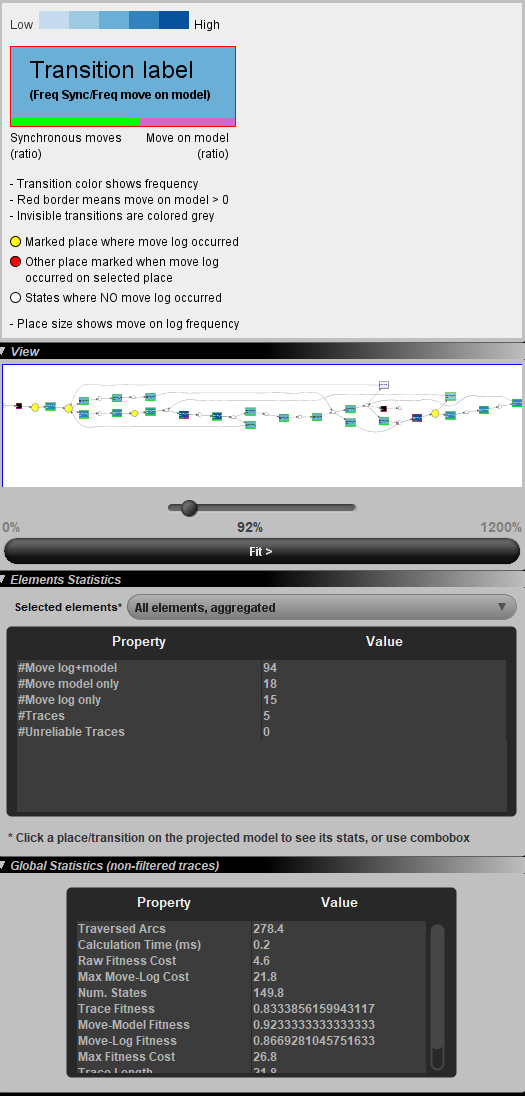
\includegraphics[width=0.3\textwidth]{MX_Papers/Paper5/images/stat1.PNG}
	   \caption{Conformance checking using ProM}
	   \label{fig:stat}
   \end{figure}
   
   
   Conformance checking is used to identify the deviation of the model by replaying a scenario on a built model. The obtained process model is compared with the event log of the same simulation model or real system. Conformance checking can be seen in two perspectives, i.e., how process model deviates from log or how event log deviates from the process model. The first one helps in fixing the process model and second one explains the error occurred in the simulation system or real system. There are several algorithms for conformance analysis like checking causal footprint, token-based replay, aligning observed and modelled behaviour, etc.
   
   
   Checking causal footprint method which is easy to compare footprint matrices of the event log with the existing reference model and fitness of the model can be measured by checking the deviation in two dependent events. This method does not consider the frequency of trace and it compares the event log with Petri net process model notation. Fitness of the model varies from value 0 to 1. If the fitness value of the process model is 1 then everything seen in the event log is possible. In order to consider frequency of trace to account, a basic token replay approach is used and it identifies the deviation and fitness by analyzing the missing and remaining token after replaying each trace on the reference process model. If there is no missing and remaining token on a modeled Petri net then there is no deviation otherwise it does not conform to the derived process model. Token replay consists of following disadvantages : All transitions in Petri net should be uniquely labeled otherwise may be it choose wrong path and give wrong measure of fitness, Token flooding is another problem because whenever there is no transition it adds more token and atlast every transition will be triggered and when local decisions about the path misleads the fitness measure won’t be reliable. Advanced method for analysing conformance is done using alignments and the problems which present in Basic token replay and checking causal footprints never occur in this method. Conformance analysis using alignments is independent of process model notation and it identifies optimal alignment using user defined cost function.
	
   
   The existing event log is added with noise and the de- rived process model is used for conformance analysis. The Replay event log on Petri net for conformance checking and its analysis given by the ProM is shown in the Figure \ref{fig:stat}. The places and transitions where the deviation occurred is explained by this method. It also provides elements statistics and global statistics which helps to get a complete picture of the deviations and other metrics like fitness of the process model. There are different plugins available in ProM which can be used for measuring precision (avoid under-fitting), generalization (avoid over-fitting), fitness (explain observed behaviour) and simplicity. There is no such thing as the best process model because each one will have a different better metric over one another. One need to identify the relevant metric for the analysis and the model which performs better in all those metrics can be selected as the appropriate model.
   
   \section{Conclusion and future work}
   \label{sec:conclusion}
   There are several applications based on process mining techniques in the field of industrial control systems. The different process discovery algorithms help to implement the model in various notations and each discovery algorithm has its own advantages and disadvantages. The appropriate model is selected by considering relevant metrics like fitness, precision, generalization, simplicity etc. The conformance checking in process mining is considered as the most important feature which identifies the deviations by comparing event log and reference model.
   
   The process model extraction using discovery algorithms and conformance checking opens a wide range of opportunities in industrial control systems. The extracted process model derived from event log can be used for the following purposes: generation of monitors in IEC 61499 standard can be used for embedding and monitoring closed-loop system in real-time \cite{wenger2015behavioral}, verification of the conformity of the control system to certified with the derived process model, real-time verification of event log to determine whether the system deviates from its actual process , re-implementing controller design and migration from legacy control systems to the IEC 61499 standard. It is possible to incorporate the process model extraction method with the IEC 61499 tool chain \cite{xavier2021cyber} for automatic verification and validation of closed-loop control systems using CTL or LTL specifications. 
   The automatic generation of plant model  from this derived reference process model could be considered as the next step in future.
   
   \section{Acknowledgements}
   This work was sponsored, in part, by the H2020 project 1-SWARM co-funded by the European Commission (grant agreement: 871743).  
   
%%% Put references here
\putbib
\end{bibunit} 